\chapter{Background \& Related Work}
In this section, I will list all technologies that are used in this project along with discussing other papers which were trying to address security with IoT devices by also trying to include blockchain technology.
\section{Legal Background}
One of the biggest motivators for this project are the recent changes in laws concerning how user data should be stored and treated. Prior to that, there was no exact limitations or regulations and companies often suffered no consequences (other than loss of trust by the customers) in case of leaking their information. This has changed severely in 2018, when General Data Protection Regulation (also known as GDPR) was introduced. Ever since lot of companies, such as Google rushed to ensure their compliance - but in the end to no avail, as both Facebook and Google suffered fines as high as \$8.8 billion on the very first day when the bill became enforceable \citep{brandom2018facebook}.

Truth is, the regulation changed the perspective on how digital industrial should be managing the information of their customers in a substantial way. First and foremost, Article 17 of GDPR, titled Right to erasure (or, `right to be forgotten'). This particular point forces all industries to allow their customers to request data erasure at any point, with no questions asked (with small exceptions, such as banking, where the data is retained because of money laundering or terrorism laws). Then, the company is forced to guarantee erasure of all logs - and if it's determined that it was not the case - face heavy fines.

The notion of Personal Identifiable Information was also put into law with special regulations on how such data should be handled. Article 4 of GDPR (titled `Definitions') describes it as:
\begin{displayquote}
‘personal data’ means any information relating to an identified or identifiable natural person (‘data subject’); an identifiable natural person is one who can be identified, directly or indirectly, in particular by reference to an identifier such as a name, an identification number, location data, an online identifier or to one or more factors specific to the physical, physiological, genetic, mental, economic, cultural or social identity of that natural person;
\end{displayquote}
Such data should either be anonymized before storing or access should be heavily audited and monitored, to minimise chance of leakage - and again, in case of non-compliance - face large fines.

Though, GDPR was only the beginning and other jurisdictions followed suit, aiming to introduce similar protections. The UK Government decided to ratified slightly modified version of GDPR into their own law and called it Data Protection Act 2018. Most recent example being state of California, introducing California Consumer Privacy Act (or CCPA for short) put into law on January 1st, 2020 \citep{CCPA}. It shared lot of similarities with GDPR and DPA, such as right to erasure, defining personal information, setting penalties and aiming to protect consumer's and their data.

\section{MQTT}
When designing architecture with the main target being the communication of many (even couple of thousands a second) clients continually exchanging data, scalability and availability needs to be kept in mind. The first and obvious solution would be to directly connect data consumers and data produces, by making them communicate in Peer-to-Peer fashion, removing the need for any extra infrastructure. This might work perfectly fine with small systems (disregarding issues such as dynamic DNS or static IP). However, as the number of clients requesting access to data increases, the total capacity of the sensor would eventually be capped - since IoT usually are of limited power and computation capacity. Imagine a scenario where a single temperature sensor continually getting bombarded with requests for current readings. It might be able to cope up to 5 incoming requests every second, everything else would cause malfunction or significantly slower response times.

Then there is also an issue of security. By allowing clients to connect to our IoT devices, we are opening a new attack vector. What if the client does not want only to access the temperature readings, but perhaps inject a worm which would intercept other sensors (such as cameras). Recently ``smart nannies'', responsible for alerting the parents when the child is crying and also relieving the adults from having to be always nearby, gained popularity. A direct camera feed could be accessed via a smartphone, no matter where. This eventually led to exploitation, as it was found that many of those devices were vulnerable to remote access by third parties\cite{pultarova2016webcam}.

MQTT aims to address those issues (and not only), by moving the communication to a separate entity, which operates in a publish-subscribe fashion. This would mean that IoT devices only have to publish information that is available to them (e.g. temperature readings), allowing to altogether remove remote access, effectively mitigating this particular attack vector. Furthermore, the MQTT brokers can be further placed behind load balancers and such to enhance their availability further.

\begin{figure}[ht]
    \centering
    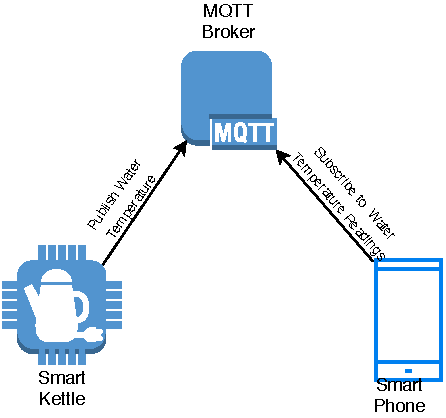
\includegraphics[width=0.5\textwidth]{mqtt_demo}
    \caption{MQTT Broker Architecture}
    \label{fig:mqtt}
\end{figure}

In short, MQTT, fully expanded to Message Queuing Telemetry Transport is an open protocol, certified by OASIS and ISO\cite{banks2019mqtt}, responsible for the publisher-subscriber architecture. It is important to point out that MQTT is not a piece of software or a server, but rather a set of standards defining what potential clients can expect (what kind of responses and data) while connection to brokers following the standard. Figure \ref{fig:mqtt} briefly shows how MQTT-compatible broker can relay information between clients. Smart Phone and Smart Kettle do not have to be online at the same time in order to receive information, nor Smart Phone is even permitted to initiate a direct connection to Smart Kettle. The broker's responsibility is to track connected subscribers (which must specify the topic of their interest) and maintain the connection until subscribe advertises session termination or abruptly disconnects (e.g. loss of power or unreliable connection).

In MQTT architecture, Client ID identifies each of the connecting entities (publisher/subscriber) and topic identifies a bridge between publishers and subscribers connected to the same topic. For example, a Smart Kettle could be publishing temperature readings under a topic called ``UK/Aberdeen/Kettle'' - then, a smartphone would need to request the same topic to receive those readings. 

\subsection{Message persistence}
This will be discussed in depth when I will describe the process of publishing and subscribing, but it is worth pointing out that by default, the messages are not saved nor cached on the broker. That is if Kettle publishes the temperature reading, but no subscribers are listening to this information, the message will perish. This is not ideal, for a situation where a smart device could wake up only every couple of minutes and then go to low-power mode again. To address this, MQTT Messages can be enriched by ``Retain'' flag. If such a flag is present, the broker will keep the message and send it straight away to any new subscribers requesting given topic. This is also useful for issuing commands to IoT devices. For example, a phone could send a command to turn off the lights with ``Retain'' flag set. Then, the smart light switch could check for retained messages every couple of minutes, removing the need for constant connection.

\subsection{Implementation}
MQTT by itself is only a collection of standards instructing implementors on what patterns should be followed and the structure of particular messages. Thus it is not shipped with any piece of software. It assumes operation on TCP layer of the network (although newer versions also allow for WebSocket support \citep{mijovic2016comparing}), thus also allowing for encrypted connection via Transport Layer Security. Every exchanged message is a TCP packet, following a strict convention- which in case of deviation is discarded as corrupted.

Two of the implementations that I have considered during this project are Mosquitto\footnote{https://mosquitto.org/} by Eclipse and Moquette\footnote{https://github.com/moquette-io/moquette}. The former written in C and the former in Java, although there is many, many more. In a paper by \citet{de2019performance}, scientists compare Moquitto and RabbitMQ, arguing their choice by the offered cloud infrastructure with more significant scalability opportunities. Moreover, some solutions are paid, whereas the considered approaches are free and open-source, allowing for a better understanding of operations. The paper is concluded with the finding that hardware and network latency has a far more significant impact on the performance, rather than the choice of the individual broker, which leaves the decision mostly down to offered extra features.

Mosquitto also offers a Docker container \cite{light2017mosquitto} in which the broker can be run, allowing for further isolation and removal of extra dependencies.

\subsection{Publishing}

The most popular method of passing MQTT messages is still under the Transport layer, as TCP packets. This allows for slightly higher freedom (compared to stricter protocols, such as HTTP), at the cost of more sophisticated parsing. MQTT standard is composed of several message types with the most important being:
\begin{itemize}
  \item CONNECT - used to initiate the connection
  \item PUBLISH - used by the client to publish messages and by the broker to publish messages to subscribers
  \item SUBSCRIBE - used by the client to request a subscription to a given topic
  \item UNSUBSCRIBE - used by the client to request removal of subscription to given topics
  \item Along with relevant *ACK counterparts (e.g. CONNACK) used to indicate the successful transmission of the message
\end{itemize}
As shown in figure \ref{fig:mqtt_publish}, the publishing flow starts with the CONNECT messages. Inside, there are several flags included, such as Quality of Service requested (MQTT can periodically send heartbeat ping to clients to check if they are still alive), requested version of MQTT protocol (at the moment, v5.0 and v3.1). This part is also referred to as ``Variable header''. The second part, known as ``Payload'' consists of the client ID.

Then, once the client has established its identity to the broker, the broker responds with CONNACK message, which contains bit informing whether a further connection is allowed or not. From this point, the client is cleared to start publishing session.

Usually, for every message to be published, there is one PUBLISH packet. A newer version of MQTT allows for spreading larger messages across multiple packets, although this will not be covered in this paper. The PUBLISH packet contains mostly two properties - topic to be published on and the actual payload. Each of the properties is prepended with 8 bytes indicating the length. From this fact, we can derive the maximum possible size of individual payload - 65535 characters (pure ASCII, no Unicode, which may take more than 1 bytes per character). Same as with CONNECT, each message is responded to with PUBACK, acting as a receipt for receiving the payload.

The client can continue to publish new messages without having to connect again, as long as the TCP session has not been terminated. Should the client want to disconnect, it should follow standard TCP flow, i.e. issue FIN/ACK packet to the broker. For situation, where the connection has been terminated abruptly, there are options such as Will flag (message to pass in case of sudden disconnection) or Keep Alive (to indicate how long should the connection be kept alive for before assuming the client has lost connection).

\begin{figure}[ht]
    \centering
    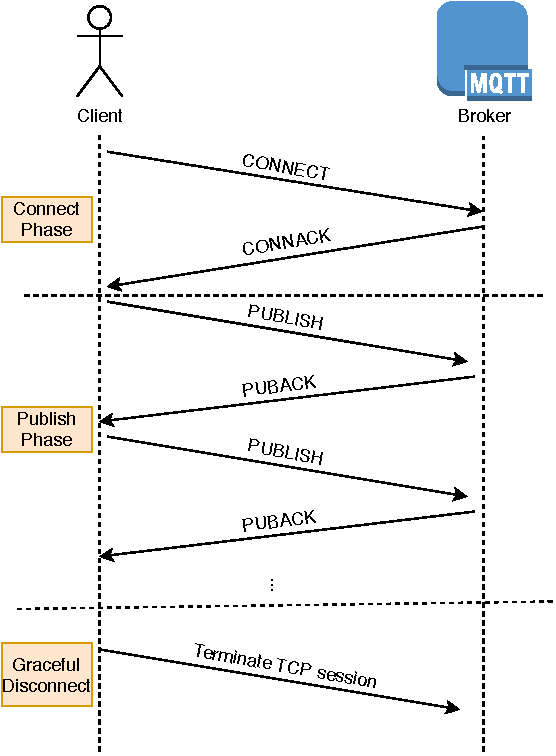
\includegraphics[width=0.6\textwidth]{mqtt_publish}
    \caption{Publishing flow with MQTT}
    \label{fig:mqtt_publish}
\end{figure}


\subsection{Subscribing}

Subscribing flow is quite similar to Publishing, with some minor differences. Following figure \ref{fig:mqtt_subscribe}, first and foremost, a connection needs to be established by instating standard TCP/TLS session and then sending CONNECT packet. The contents follow the same standard, i.e. containing information such as Client ID or even optional parameters in the form of ``key: value'' (particularly useful for this project).

\begin{figure}[ht]
    \centering
    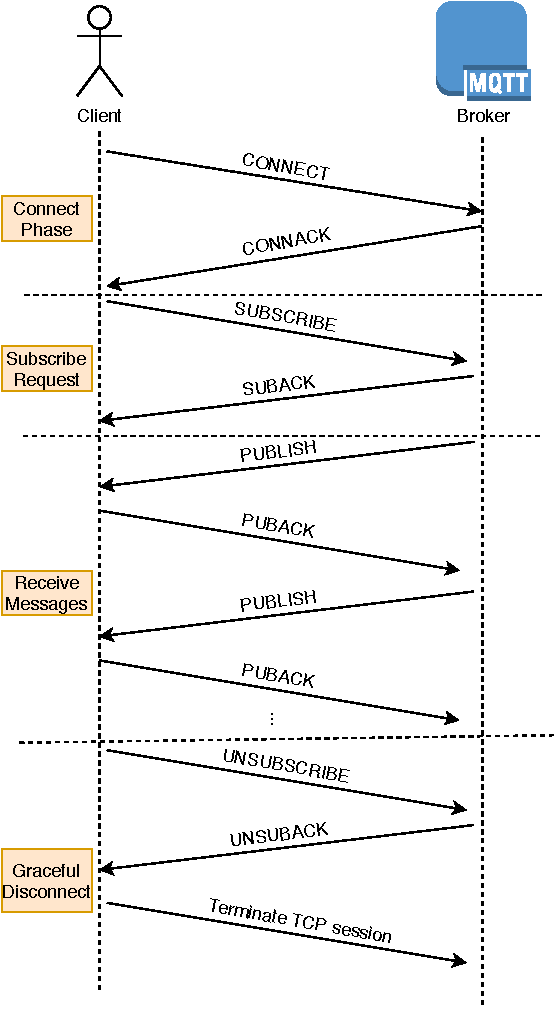
\includegraphics[width=0.6\textwidth]{mqtt_subscribe}
    \caption{Subscribing flow with MQTT}
    \label{fig:mqtt_subscribe}
\end{figure}

After a successful connection, the client can proceed to send a request for subscription. Similar with PUBLISH packet, the client specifies the type of the packet in the variable header and then requested topic for subscription in the payload. The extra element is the QoS flag - Quality of Service. MQTT has three levels of QoS:
\begin{enumerate}
  \item 0 - No response to PUBLISH messages
  \item 1 - PUBLISH messages will be followed by PUBACK
  \item 2 - More granular control over PUBLISH, with extra packets such as PUBREC (Publish Received), PUBREL (Publish Release) and PUBCOMP (Publish Complete).
\end{enumerate}

Once the SUBSCRIBE message has been processed and approved by the broker, it will issue SUBACK message and remain connected to the client. From this point, any message that is published on the topic specified in SUBSCRIBE packet will be published (as PUBLISH packet) to every client currently subscribed to it. Of course, depending on requested QoS, the broker might then await for PUBACK message (or even issue other messages such as PUBREC, PUBREL, PUBCOM). The diagram demonstrates a simple exchange with QoS set to 1. 

\begin{table}[]
\centering
\begin{tabular}{llllllllllllll}
\hline
\multicolumn{1}{|l|}{82} & \multicolumn{1}{l|}{04} & \multicolumn{1}{l|}{00} & \multicolumn{1}{l|}{01} & \multicolumn{1}{l|}{00} & \multicolumn{1}{l|}{07} & \multicolumn{1}{l|}{F} & \multicolumn{1}{l|}{L} & \multicolumn{1}{l|}{Y} & \multicolumn{1}{l|}{T} & \multicolumn{1}{l|}{R} & \multicolumn{1}{l|}{A} & \multicolumn{1}{l|}{P} & \multicolumn{1}{l|}{00} \\ \hline
1                        & 2                       & 3                       & 4                       & 5                       & 6                       & 7                      & 8                      & 9                      & 10                     & 11                     & 12                     & 13                     & 14                     
\end{tabular}
\caption{Example SUBSCRIBE to topic FlyTrap packet}
\label{tab:sub_packet}
\end{table}

To close off MQTT, I also wanted to overview an example packet and dissect it byte by byte to demonstrate exactly what kind of information is included - this can be seen in table \ref{tab:sub_packet}
\begin{enumerate}
  \item [1] Control field, specifies the type of the message (CONNECT, SUBSCRIBE etc.)
  \item [2] Remaining length of the message. Can be expanded to 2 bytes.
  \item [3-4] Packet ID
  \item [5-6] Payload length
  \item [7-13] Payload. Corresponding hex encoding of characters, replaced with actual characters for clarity
  \item [14] Requested QoS
\end{enumerate}

\section{Blockchain}

Lots of concepts in this paper involve blockchain methodologies, which, by itself, is an expansive area. As part of this section, I will be only covering the most relevant topics necessary to understand the design choices taken within my project, but further reading is strongly encouraged.

\subsection{Architecture}
Blockchain often goes by its infamous name of simply overly complicated linked-list, and in fact, it is not very far away from being true. The concept was first introduced and popularised by \citet{nakamoto2008peer} in a paper introducing a highly controversial notion of digitalising and decentralising currency, by moving it into a structure called a blockchain. Blockchain network was meant to operate on a peer-to-peer basis, with different peers validating each other's transactions and holding a copy of the entire block. This removes the need for a central authority governing the currency (for example, central banks), by placing a copy of all records on every participant's computer - one problem remained, and that was trust. How do we trust other peers that they do not inject fraudulent transactions? However, before I answer this question, let us focus on figure~\ref{fig:blockchain}, which outlines the difference between distributed and centralised ledgers. With the current economic model, usually there exist some central authority (in this example, a central bank) which is responsible for tracking, verifying and authorising all transactions between participants. Compare it with a decentralised ledger, where there is no such central entity. Instead, each participant verifying all transactions that happen between nodes. They no longer have to trust Central Bank to do their job currently, as they are free to confirm the authenticity of all transactions themselves. Nevertheless, again, we get back to the same question - how does the authentication happen?

\begin{figure}[ht]
    \centering
    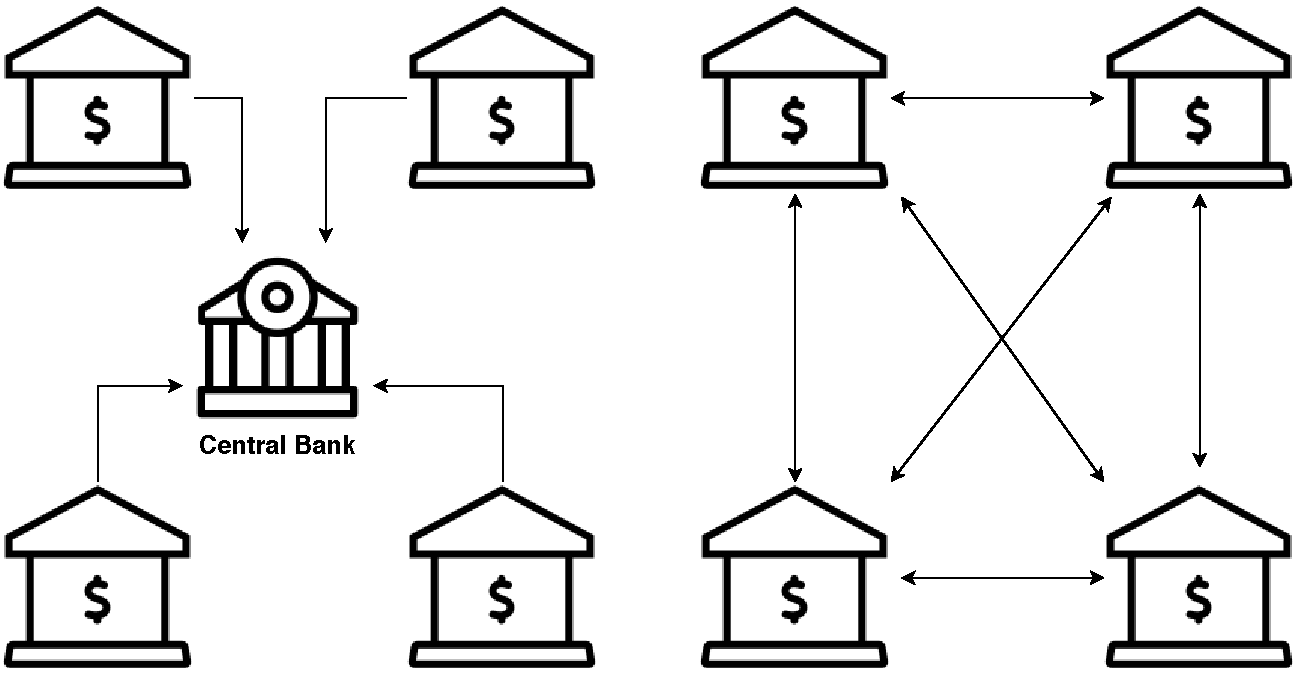
\includegraphics[width=0.7\textwidth]{blockchain}
    \caption{Centralised Ledger (on the left) vs Decentralised Ledger (on the right)}
    \label{fig:blockchain}
\end{figure}

\subsection{Consensus Algorithms \& Proof-of-Work}
Before a participant can add their transaction (``block'' from blockchain) to the public records (``chain'' from blockchain), we need a cryptographically secure mean to verify whether this particular participant can add this block. Establishing trust between participants on a blockchain is often referred to as ``consensus''. Thus, several consensus algorithms exist. Currently, perhaps the most popular one, it is proof-of-work. In fact, PoW dates even before the paper by Satoshi Nakamoto, all the way back to \citet{jakobsson1999proofs}. It utilises one of the most critical properties of hash functions, that is pre-image resistance. The blockchain will offer a cryptographic puzzle to the participant willing to add a new block. This puzzle would be based on reversing a hash, i.e. a hash would be generated, and the participant would be tasked with reversing it, thus getting the original value. This ``puzzle'' is also often referred as mining a new block, that is, finding a value that after passing through specified hash function would produce expected output (also known as cracking hashes) - that is also part of the reason why modern mining requires much computational power. 

Then, everyone starts a race towards reversing this hash. The first person to achieve the target is rewarded with a possibility to add new a block to the network (along with the found value). In the future, any peer can verify the authenticity by feeding the attached value through the hash function and verifying whether the obtained value matches the expected hash. All of it is possible since computing hashes is relatively fast and not a very computationally expensive operation. At the very end, when attaching the new block to the chain, the miner is usually rewarded with cryptocurrency, which can then later be exchanged with other participants.

\begin{figure}[ht]
    \centering
    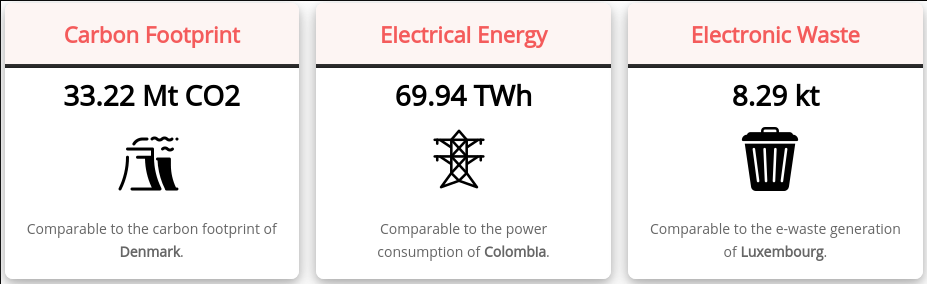
\includegraphics[width=0.9\textwidth]{footprint}
    \caption{Annualized Total Footprint of Bitcoin network \cite{index2017digiconomist}}
    \label{fig:footprint}
\end{figure}

Of course, this approach has several downsides. First of all, all the computational power is effectively wasted to this cryptographic puzzle, with no real end-use - especially if you take part in the race to crack the next hash and someone ends up being faster than you - all your effort went for nothing. This was widely discussed by scientists \cite{gervais2016security}, who currently point out a negative impact on the environment. As reported by portal Digiconomist \cite{index2017digiconomist}, as of 2020, the annualised carbon footprint of Bitcoin network can be compared with the carbon footprint of the entire country of Denmark, with extra samples such as electrical consumption or electronic waste in figure~\ref{fig:footprint}

Another problem that Proof-of-Work algorithms create is a $51\%$ attack. Nowadays, setting up your Bitcoin node and starting to mine is not very feasible since people with higher hash rates (the speed at which a person can crack hashes) usually form organisations, that share this power amongst each other and then once they can crack the individual hash, reward each of the members with only a small portion. This might sound good for individuals since now they are guaranteed a payout (rather than risking taking part in the race and losing, winning nothing), but it effectively defeats the decentralised concept of blockchain. If one organisation holds more than $51\%$ of the hash rate of the entire blockchain, it can start authorising fraudulent blocks and adding them to the chain. Since they hold the majority of the network's hash rate, nobody can defy them. 

\begin{figure}[h]
    \centering
    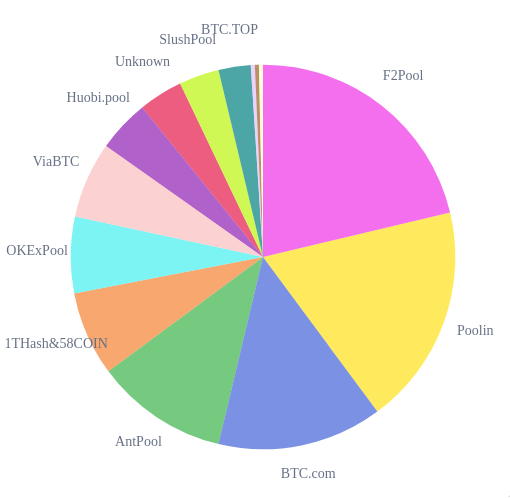
\includegraphics[width=0.5\textwidth]{51}
    \caption{Summary of Mined Blocks as of 2020-03-30, per blockchain.com}
    \label{fig:51}
\end{figure}

Figure~\ref{fig:51} shows the approximate split of total mined blocks in the past 48hrs since March 30th. Now, imagine a situation where organisations BTC.com, Proolin and F2Pool started collaborating, taking over 51\% of the market. They would be able to add arbitrary blocks, self-verifying them - and since they hold the majority, nobody could oppose it.
\subsection{Proof-of-Stake}
A slightly different approach to verifying the transaction is called proof-of-stake, first introduced by \cite{king2012ppcoin} - which does not involve cryptographic puzzles nor requires high computational power and is all based on some pre-defined amount of cryptocurrency that is being put on hold, while delegates are selected. Every participant can bet any amount of crypto - which is returned to them after the validator is selected. The process can be outlined in the following steps:
\begin{enumerate}
    \item Participants define their stake.
    \item Network selects one participant that is going to be acting as a validator for the next block. The higher the stake, the higher the chance of getting selected. Losers get their stake back.
    \item validator goes ahead and verifies the next block gets added to the chain, there is no block reward, although they receive network fees for the transaction.
    \item After a couple of days (once other participants verify the transaction was not fraudulent), the stake is released and goes back to the validator.
\end{enumerate}
This partially eliminates the issue of $51\%$ attack mentioned above. First, because hash rate nor computational power no longer matters (and thus forming organisations loses the point) and secondly, even if the fraudster held more than half of the entire markets crypto, they would still be at risk of losing the stake, as their chance of getting selected as a validator is not 100\%.

Sadly, this approach also is not free of any issues. Contrary to what I mentioned above, it creates a bias towards participant with more significant wealth, which can put more value on stake. This might create situations where rich get richer - though there is always a non-zero chance of getting selected. Furthermore, while they might not have malicious intents, they would be at a higher chance of getting selected as validator and thus collecting more network fees.

As this field is still expanding, more work is published, suggesting refined approaches. At the current day, both Bitcoin and Ethereum use Proof-of-Work, though the latter aims to move towards Proof-of-Stake in the future iterations \cite{saleh2020blockchain}.
\subsection{Proof-of-Authority}
However, what if we do not care about full decentralisation and want to avoid extra operational costs through proof-of-work or proof-of-stake algorithms? A simpler solution, called proof-of-authority \cite{network2017proof} can also be used. This approach offers no rewards for adding new blocks to the chain, so it is not used in public blockchains. The validators are pre-selected and are responsible for vetting new blocks. This has more uses in situations where data does not have to remain secret, and we do not mind the lack of decentralisation. In fact, if the validators become compromised, they would be able to start allowing malicious blocks.
\subsection{Ethereum}
Proof-of-Work proved itself to be a tremendous waste of energy and resources, with Bitcoin using it solely for authorising the transaction and nothing beyond it. That particular period was also a time when a lot of different currencies started showing up, as Bitcoin's source code was open, everybody was allowed to host their network. Ethereum was one of them, but it was also the first to introduce a concept known as smart-contracts - a way to put the proof-of-work energy to some use (though still a lot of was wasted), introduced in 2015 by \citet{buterin2014ethereum}. The network also gave birth to so-called decentralised applications (or Dapps for short), through smart-contracts. Smart-contract can be understood as pieces of code which can get executed on the blockchain, written in a specialised language called Solidity inside EVM (Ethereum Virtual Machine). The transactions were no longer limited to the information about transferring currency between accounts, but also could execute code and act as a persistent database, which could not be altered by anyone and change history was publicly available.


\section{IoT, Hyperledger and GA}

Attempts at combining IoT authorisation with blockchain has been made in the past. One of the examples is a recent work by scientists from Khon Kaen University in Thailand. In that paper \cite{klaokliang2018novel}, researchers look into Authorization Architecture for IoT (using MQTT broker as an intermediary entity). They are arguing about the benefits of combining any solutions for low-power devices and distributed architecture, which ultimately enables much better scalability and removes the single point of failure.

They are also utilising Hyperledger Fabric - another blockchain-based ledger. Compared to Ethereum, Hyperledger \cite{cachin2016architecture} is used mostly for Business-to-Business scenarios, as it does not feature any reward for mining, i.e. adding extra blocks to the chain. Transparency is also limited, as the information is no longer placed on a publicly available platform but rather depends on trusting the nodes connect to the network although I will spend some more time discussing differences in implementation and discussion chapters of this paper.

Moreover, the focus of that paper is at finding optimised consensus algorithm, such that any latency caused by permission lookup is minimised. Scientists suggest using Genetic Algorithms to compose Optimal Consensus. Their experiments were executed on Kafta MQTT\cite{waehner_2019}. Thai researchers were able to achieve the performance of their solution called GA Kafka improved by 69.43\% compared to standard Kafka.

Although this paper does not take into consideration other parts of the AAA framework, focusing solely on Authorisation. It has no mention of authenticating connecting clients or making them accountable by keeping audit crumbs of the most sensitive operations conducted on the chain. In my work, I will also be less focus on the performance of the blockchain network itself, leaving this down to the blockchain itself. As mentioned in the previous section, Ethereum has had some rapid movements in terms of improving their consensus algorithms and moving away from Proof-of-Work instead aiming to implement Proof-of-Stake.
